\documentclass[a4paper, 12pt]{report}
\usepackage{hyperref}
\usepackage{blindtext}
\usepackage{indentfirst}
\usepackage{graphicx}
\usepackage{xcolor}
\usepackage{array}
\usepackage{tikz}

\graphicspath{ {./images/} }
\definecolor{ao(english)}{rgb}{0.0, 0.5, 0.0}
\def\checkmark{\tikz\fill[scale=0.4](0,.35) -- (.25,0) -- (1,.7) -- (.25,.15) -- cycle;} 

\hypersetup{
    colorlinks=true,
    linkcolor=black,   
    urlcolor=cyan,
}

\begin{document}
    \begin{titlepage}
        \begin{center}
            {\huge\textbf{Project proposal}}

            \vspace{0.25cm}
            {\large\textbf{Crowd quizmaker}}

            \vspace{1cm}
            by
                
            \vspace{0.25cm}
            \textbf{0N3 N16H7 PR0J3C7}

            \vspace{0.25cm}
            Suwat Inkaew 610610521

            Kritsanaphong Tepweerakul 630610714

            Kitpisan Tanngan 630610716

            Chayanon Pitak 630610724

            Nadtaphong Jandaboot 630610743

            Woranut Kitchakan 630610760

            \vspace{1cm}

            \href{https://github.com/ChayanonPitak/261361-Project/}{https://github.com/ChayanonPitak/261361-Project/}
        \end{center}
    \end{titlepage}

    \tableofcontents

    \pagebreak
    \addcontentsline{toc}{section}{Team profile}
    \section*{Team profile}
        \begin{itemize}
            \item \textbf{Chayanon Pitak} as Project Manager and System Analyst
            
                \textbf{Skills}
                \begin{itemize}
                    \item \textbf{Web application development} on JavaScipt, Typescript, React.js, Solid.js, PHP, TailwindCSS.
                    \item \textbf{Software development} on Java, C, C++.
                    \item \textbf{Game development} on Unity using C\#.
                \end{itemize}

                \textbf{Experience}
                \begin{itemize}
                    \item Mostly college projects and personal projects.
                \end{itemize}
            \item \textbf{Kritsanaphong Tepweerakul} as Developer and Business Analyst
                
                \textbf{Skills}
                \begin{itemize}
                    \item \textbf{Web application development} on JavaScipt, Typescript, React, TailwindCSS, PHP, Laravel.
                    \item \textbf{Software development} on C, C++, C\#, Java, Python.
                    \item \textbf{Game development} on Spring boot/React Web-based Game, Unity.
                \end{itemize}
                
                \textbf{Experience}
                \begin{itemize}
                    \item SFML 2D-RPG Game.
                    \item CARIN. (Strategy-Game Project)
                    \item Gogoboard Automatic Watering.
                    \item Store Website.
                \end{itemize}

                \item \textbf{Woranut Kitchakan} as Developer and Designer

                \textbf{Skills}
                \begin{itemize}
                    \item \textbf{Web application development} on JavaScipt, Typescript, React, TailwindCSS, Laravel.
                    \item \textbf{Software development} on C++, Java.
                    \item \textbf{Game development} on C++, Spring boot/React Web-based Game.
                \end{itemize}

                \textbf{Experience}
                \begin{itemize}
                    \item SFML Platform games.
                    \item CARIN. (Strategy-Game Project)
                    \item Gogoboard Automatic clothes drying machine.
                \end{itemize}

            \item \textbf{Kitpisan Tanngan} as Tester and Designer
                \textbf{Skills}
                \begin{itemize}
                    \item \textbf{Web application development} on JavaScipt, Typescript, React, TailwindCSS, Laravel.
                    \item \textbf{Software development} on  C++, Java.
                    \item \textbf{Game development} on C++, Java.
                \end{itemize}
            
                \textbf{Experience}
                \begin{itemize}
                    \item Turn-base Game Project.
                    \item Gogoboard Automatic roof for plants.
                \end{itemize}

            \item \textbf{Nadtaphong Jandaboot} as Tester and Designer
            
                \textbf{Skills}
                \begin{itemize}
                    \item \textbf{Web application development} on TailwindCSS.
                    \item \textbf{Software development} on C++.
                    \item \textbf{Art and Editing} on Photoshop. 
                \end{itemize}

                \textbf{Experience}
                \begin{itemize}
                    \item Mostly a art designer and sometimes front-end developer in projects. 
                \end{itemize}

            \item \textbf{Suwat Inkaew} as Tester
            \textbf{Skills}
                \begin{itemize}
                    \item \textbf{Web application development} on a little bit of JavaScipt, Typescript, React, TailwindCSS.
                    \item \textbf{Software development} on C, C++ and a little bit of C\#, Java.
                \end{itemize}
                
                \textbf{Experience}
                \begin{itemize}
                    \item SCRATCH Game.
                    \item CARIN(Tower Defense Game).
                    \item Review Website.
                    \item Card Game Project.
                \end{itemize}

        \end{itemize}

    \pagebreak
    \addcontentsline{toc}{section}{About project}
    \section*{Crowd quizmaker}
    Students and lecturers generate quiz and answers. Quizzes can be edited, commented, voted and rated (e.g. quiz-maker)

    \addcontentsline{toc}{section}{Problem statement}
    \section*{Problem statement}
    
    Nowadays "Social network" is very popular for people to hang out on, they can see what their follower are doing, they can interact with follower and they can share their own content.

    But there is no "Examination Social Network" yet. Which can be a way to evaluate student's knowledge and let them to compete with each other that also fun for the student. For example, in the past Internet and Online Community course (261111) have a traditional examination, which is boring and not interactive. But if we have a "Examination Social Network" that can be a way to evaluate student's knowledge and let them to compete with each other that also fun for the student.
    
    \pagebreak
    \addcontentsline{toc}{section}{Solution}
    \section*{Solution}

    \subsection*{Facebook group}
    \begin{center}
        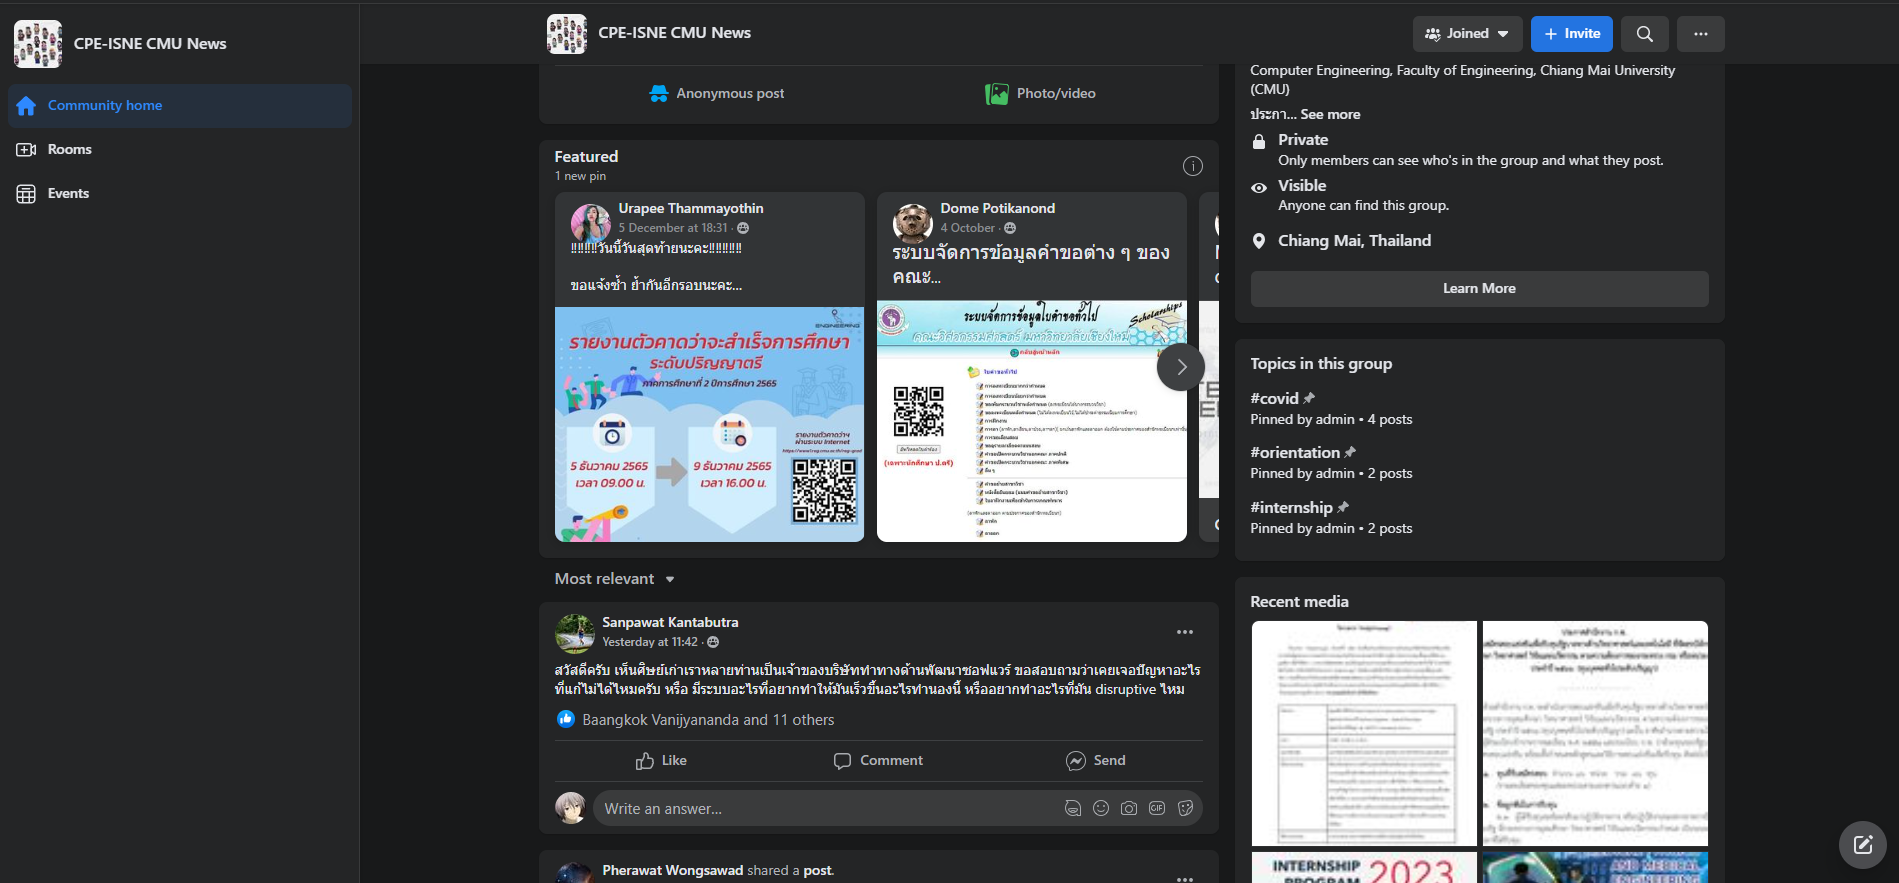
\includegraphics[height=150px]{facebook_group.png}
    \end{center}

    \textbf{Facebook group} is a group platform created by Meta. It let people with same interest to gather or lecturer can communicate with student. Also it is a way to let people create post (including quiz) and interact with each other. But it cannot evaluate student performance nor quiz quality and managing posts into topics/quizes is very hard or impossible to do.

    \subsection*{Quiz-maker}
    \begin{center}
        
\includegraphics[height=150px]{quiz-maker.png}
    \end{center}
    
    \textbf{Quiz-maker} is a quiz creation platform. User can create quizzes of their own topic and share to others. It have great evaluation but lack of interaction and quizzes quality review from other users is impossible.
    
    
    \subsection*{Kahoot!}
    \begin{center}
        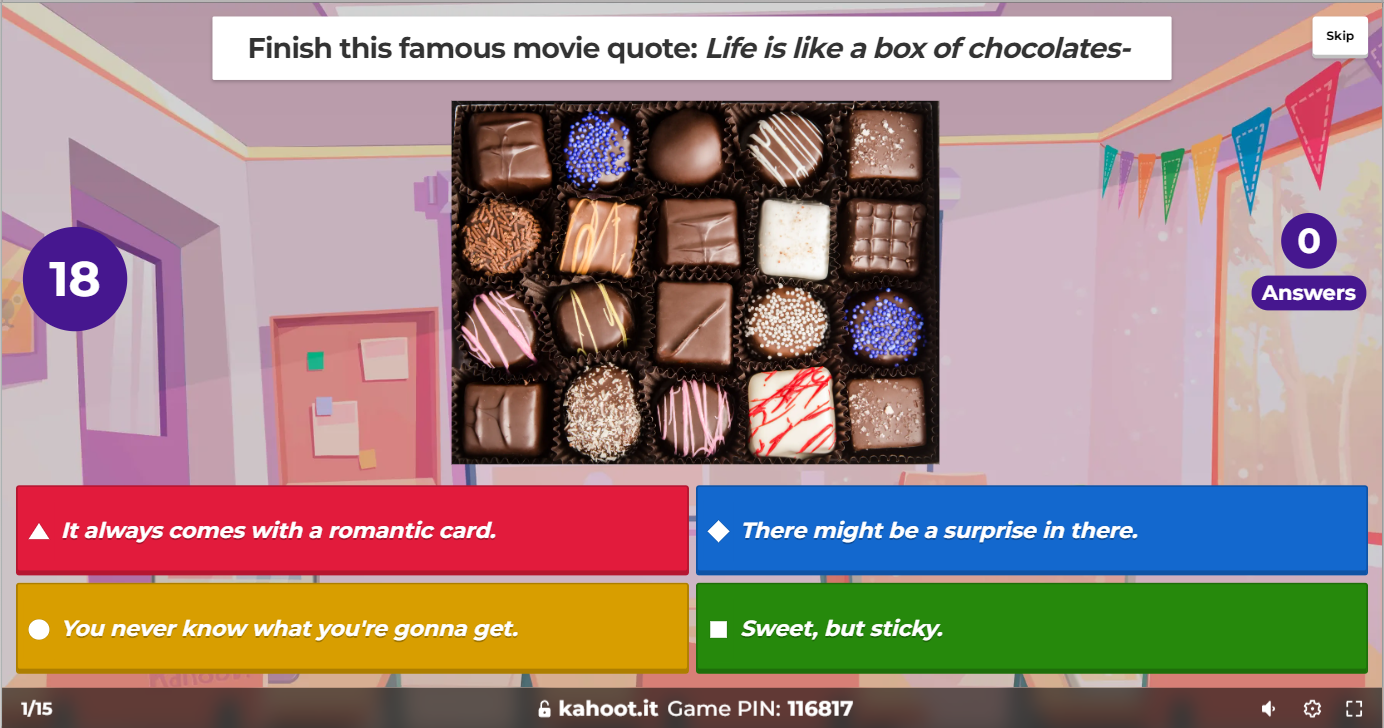
\includegraphics[height=150px]{kahoot.png}
    \end{center}
    
    \textbf{Kahoot} is a game-based learning platform. It let lecturer create questions according to topics and student can syncronously answer the questions with intensive environment. It have great evaluation and fun. But students cannot contribute their own quiz to existing quizzes.

    \subsection*{Learning managament syatems (LMS) - Moodle, Blackboard, Canvas, etc.}
    \begin{center}
        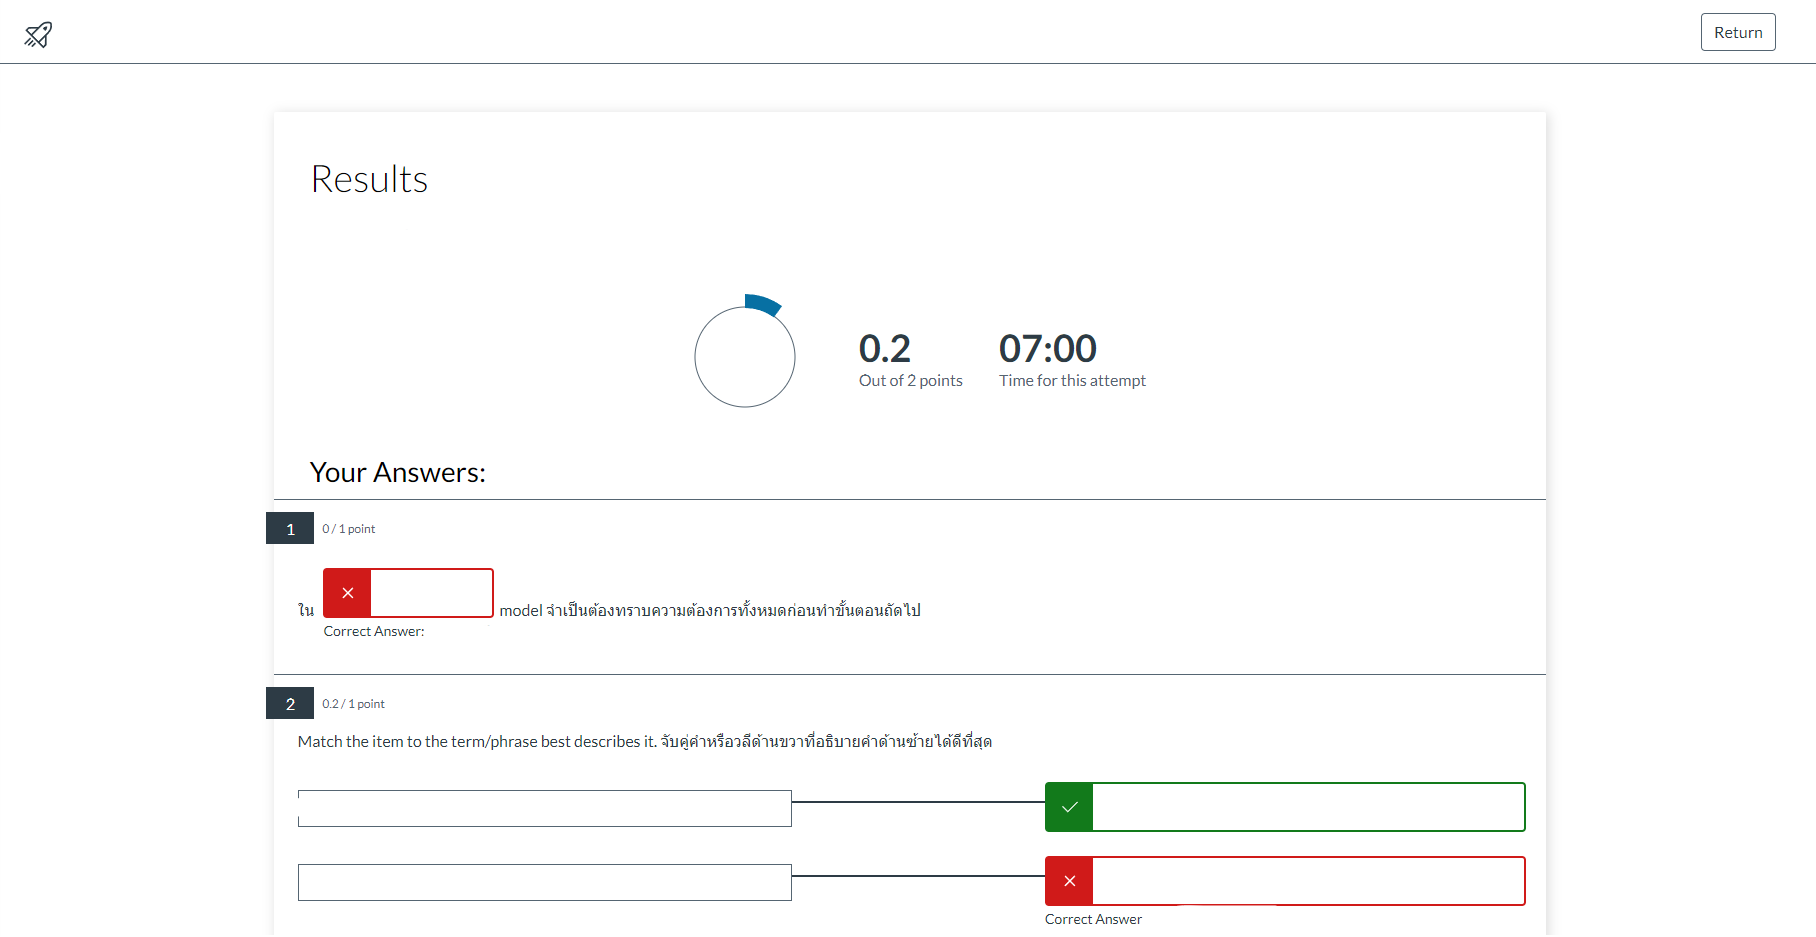
\includegraphics[height=150px]{LMS.png}
    \end{center}

    \textbf{Learning management system (LMS)} is an application that automates the administration, tracking, and reporting of training events.\footnote{Ryann K. Ellis, Field Guide to Learning Management Systems, Learning Circuits, 2009, p.1} It have great evaluation and grading, but quizzes looks like traditional examination.

    \pagebreak
    \addcontentsline{toc}{section}{Contribution}
    \section*{Contribution}

    In general, quiz is created by one person or one group. It makes the number of quiz and variety of quiz is low. We have an inspiration of Facebook group which everyone in the groups can contribute to a topic, which will increase the variety and number of quiz. The process of creating quiz is as follows: define questions, define choices, define correct answers, have a system that can comment or vote on the quiz created by others to review the quality and correctness of the quiz, have a system that can evaluate the quality of the quiz.

    \addcontentsline{toc}{subsection}{Contribution to existing solutions}
    \subsection*{Comparison to existing solutions}
    
    \begin{itemize}
        \item Facebook groups
        \begin{center}
            \begin{tabular}{| m{10em} | m{12em} | m{12em} |}
                \hline
                 & Facebook group & Our solution \\ 
                \hline\hline
                Quiz creation & Creating posts & \textcolor{ao(english)}{Creating quizzes with defined format} \\  
                \hline
                Quiz contribution & Everyone in group or group moderator approval & \textcolor{ao(english)}{Defined by subject creator} \\
                \hline
                Quiz validation & - & \textcolor{ao(english)}{Pre-defined format} \\
                \hline
                Quiz quality review & Reactions and Comments & \textcolor{ao(english)}{Pre-defined rubrics} \\
                \hline
                User evaluation & Manually & \textcolor{ao(english)}{User dashboard} \\
                \hline
            \end{tabular}
        \end{center}

        \item Quiz-maker
        \begin{center}
            \begin{tabular}{| m{10em} | m{12em} | m{12em} |}
                \hline
                 & Quiz-maker & Our solution \\ 
                \hline\hline
                Quiz creation & \textcolor{ao(english)}{Creating quizzes with defined format} & \textcolor{ao(english)}{Creating quizzes with defined format} \\  
                \hline
                Quiz contribution & Quiz creator & \textcolor{ao(english)}{Defined by subject creator} \\
                \hline
                Quiz validation & \textcolor{ao(english)}{Pre-defined format} & \textcolor{ao(english)}{Pre-defined format} \\
                \hline
                Quiz quality review & - & \textcolor{ao(english)}{Pre-defined rubrics} \\
                \hline
                User evaluation & \textcolor{ao(english)}{User dashboard} & \textcolor{ao(english)}{User dashboard} \\
                \hline
            \end{tabular}
        \end{center}

        \pagebreak
        \item Kahoot!
        \begin{center}
            \begin{tabular}{| m{10em} | m{12em} | m{12em} |}
                \hline
                 & Kahoot! & Our solution \\ 
                \hline\hline
                Quiz creation & \textcolor{ao(english)}{Creating quizzes with defined format} & \textcolor{ao(english)}{Creating quizzes with defined format} \\  
                \hline
                Quiz contribution & Quiz creator & \textcolor{ao(english)}{Defined by subject creator} \\
                \hline
                Quiz validation & \textcolor{ao(english)}{Pre-defined format} & \textcolor{ao(english)}{Pre-defined format} \\
                \hline
                Quiz quality review & Stars rating & \textcolor{ao(english)}{Pre-defined rubrics} \\
                \hline
                User evaluation & \textcolor{ao(english)}{User dashboard} & \textcolor{ao(english)}{User dashboard} \\
                \hline
                Syncronous activity & \textcolor{ao(english)}{\checkmark} & \textcolor{ao(english)}{\checkmark} \\
                \hline
            \end{tabular}
        \end{center}

        \item Learning management system
        \begin{center}
            \begin{tabular}{| m{10em} | m{12em} | m{12em} |}
                \hline
                 & LMS & Our solution \\ 
                \hline\hline
                Quiz creation & \textcolor{ao(english)}{Creating quizzes with defined format} & \textcolor{ao(english)}{Creating quizzes with defined format} \\  
                \hline
                Quiz contribution & Quiz creator  & \textcolor{ao(english)}{Defined by subject creator} \\
                \hline
                Quiz validation & \textcolor{ao(english)}{Pre-defined format} & \textcolor{ao(english)}{Pre-defined format} \\
                \hline
                Quiz quality review & - & \textcolor{ao(english)}{Pre-defined rubrics} \\
                \hline
                User evaluation & \textcolor{ao(english)}{User dashboard} & \textcolor{ao(english)}{User dashboard} \\
                \hline
            \end{tabular}
        \end{center}
    \end{itemize}

    \pagebreak
    \addcontentsline{toc}{section}{Stakeholder and User groups}
    \section*{Stakeholder and User groups}
        \begin{itemize}
            \item \textbf{Product Owner}
            \begin{itemize}
                \item Professor Kampol Woradit as Internet and Online Community course lecturer. 
                \item Professor Sakgasit Ramingwong as Internet and Online Community course lecturer. 
            \end{itemize}
            \item \textbf{Study purpose}
            \begin{itemize}
                \item Lecturers
                \item Students
            \end{itemize}
            \item \textbf{Entertain purpose}
            \begin{itemize}
                \item Quiz Makers
                \item Who want to take advantage from their free time
                \item Who is interested in specific purpose
                \item Content creater who want to created content based on fan-quizzes
            \end{itemize}
        \end{itemize}
    

    \pagebreak
    \addcontentsline{toc}{section}{Technology feasibility study}
    \section*{Technology feasibility study}
    We will create web application which is cross-platform friendly that can be use on mostly any device.

    \addcontentsline{toc}{subsection}{Tool and resources used}
    \subsection*{Tool and resources used}
    \begin{itemize}
        \item Figma for UI/UX design.
        \item Swagger for API design.
        \item diagrams.net for database design.
        \item HTML/CSS for web markdown and styling.
        \item Typescript for backend
        \item React.js for frontend framework.
        \item MySQL for database system.
        \item Prisma for database orm.
    \end{itemize}


    \pagebreak
    \addcontentsline{toc}{section}{Conclusion}
    \section*{Conclusion}

    We will create cross-playform web application that's looks like combination of Facebook groups and LMS, which lets user gather in groups and create quizzes together. Also users can review and rated quizzes quality.

    We will separete into two user groups.
    \begin{itemize}
        \item For \textbf{Lecturer and student}, lecturer can create and subject topic and let student create quizzes related to that topic. After that student will take each other quizzes to test their knowledge and rate their quizzes quality. This method make the quizzes become larger and more accurate for that subjects that student also have fun.
        \item For \textbf{Fans}, they can create quizezs related to their favorite topic and let others to contribute that topic.
    \end{itemize}

    \pagebreak
    \addcontentsline{toc}{section}{Appendix}
    \section*{Appendix}
        \addcontentsline{toc}{subsection}{A1 - responsibility}
        \subsection*{A1 - responsibility}
        \begin{itemize}
            \item \textbf{Suwat Inkaew 610610521} (2\%) - Self profile.
            \item \textbf{Kritsanaphong Tepweerakul 630610714} (41.58\%) - Self profile, Stakeholder interview (Proj. Kampol Woradit), Contribution section, Stake holder and User groups section.
            \item \textbf{Kitpisan Tanngan 630610716} (2\%) - Self profile.
            \item \textbf{Chayanon Pitak 630610724} (50.42\%) - Document setup, Self profile, Stakeholder interview (Prof. Sakgasit Ramingwong), Problem defination, Alternatives purpose, Technology defination, Conclusion.
            \item \textbf{Nadtaphong Jandaboot 630610743} (2\%) - Self profile.
            \item \textbf{Woranut Kitchakan 630610760} (2\%) - Self profile.
        \end{itemize}

        \addcontentsline{toc}{subsection}{A2 - Responsibility percentage calculation}
        \subsection*{A2 - Responsibility percentage calculation}

        Activities that not directly contribute to the documentclass
        \begin{itemize}
            \item Stakeholder interviewing 10\%
        \end{itemize}
        Activities that is directly contribute to the documentclass
        \begin{itemize}
            \item Document setup 0\%
            \item Self profile 2\%
            \item Other large section ~8.86\%
        \end{itemize}
    
\end{document}